\begin{frame}
    \frametitle{\problemtitle}
    \begin{block}{Problem}
        Given a binary tree, determine the minimal number of leaves you should remove to make the tree strongly balanced.
    \end{block}
    \pause
    \begin{block}{Solution}
        \begin{itemize}
            \item<+-> Every vertex should be balanced: the height of its left and right subtree should differ by at most one.
            \item<+-> Naive solution: remove the deepest leaves below vertices that are too high.
            \item<+-> This takes $\mathcal{O}(n)$ time per vertex, so too slow.
        \end{itemize}
    \end{block}
\end{frame}
\begin{frame}
    \frametitle{\problemtitle}
    \begin{block}{Problem}
        Given a binary tree, determine the minimal number of leaves you should remove to make the tree strongly balanced.
    \end{block}
    \begin{block}{Solution}
        \begin{itemize}
            \item<+-> Idea: determine the maximal height every subtree can have,
                and then remove vertices.
            \item<+-> First, compute all heights using a DFS.
            \item<+-> Set the required heights using a second DFS. For a vertex $v$ with children $l$ and $r$, the minimal required height of $l$ is: $\min(H(l),H(r)+1,ReqH(v)-1)$. Analogous for $r$.
            \item<+-> Finally, remove all vertices with negative height.
            \item<+-> Runtime: $\mathcal{O}(n)$
        \end{itemize}
    \end{block}
\end{frame}

\begin{frame}
    \frametitle{\problemtitle}
	\begin{block}{Problem}
        Given a binary tree, determine the minimal number of leaves you should remove to make the tree strongly balanced.
    \end{block}

    \vspace{-0.2cm}
    \begin{overprint}
		\onslide<1>
		\centering
		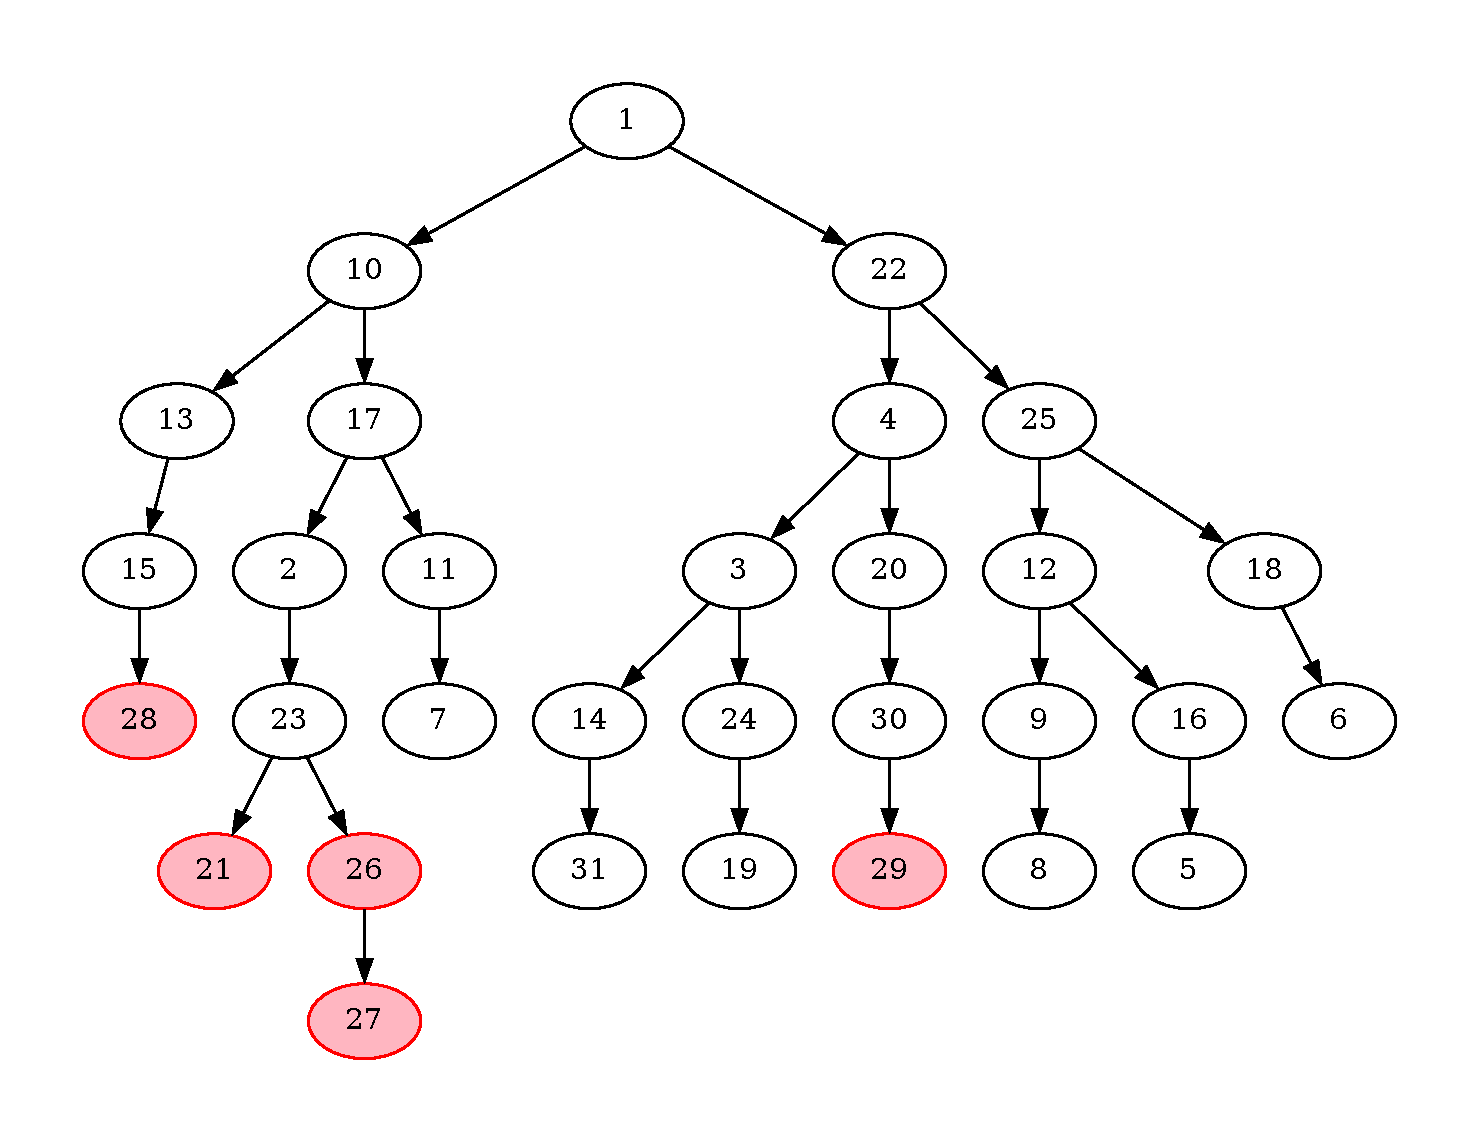
\includegraphics[height=0.65\textheight]{./visuals/1}
		\onslide<2-3>
		\centering
		
\includegraphics[height=0.65\textheight]{./visuals/2}
	\end{overprint}
    \pause
	\solvestats
\end{frame}
